\documentclass[a4paper, 11pt]{article}
\usepackage{comment} % enables the use of multi-line comments (\ifx \fi) 
\usepackage{fullpage} % changes the margin
\usepackage[a4paper, total={7in, 10in}]{geometry}
\usepackage{amsmath,mathtools,mathdots}
\usepackage{amssymb,amsthm}  % assumes amsmath package installed
\usepackage{float}
\usepackage{xcolor}
\usepackage{mdframed}
\usepackage[shortlabels]{enumitem}
\usepackage{indentfirst}
\usepackage{hyperref}
\hypersetup{
	colorlinks=true,
	linkcolor=doc!80,
	citecolor=myr,
	filecolor=myr,      
	urlcolor=doc!80,
	pdftitle={Assignment}, %%%%%%%%%%%%%%%%   WRITE ASSIGNMENT PDF NAME  %%%%%%%%%%%%%%%%%%%%
}
\usepackage[most,many,breakable]{tcolorbox}
\usepackage{tikz}
\usepackage{caption}
\usepackage{mathpazo}
\usepackage{libertine}
\usepackage{physics}
\usepackage[ruled,vlined]{algorithm2e}
\usepackage{mathrsfs}
\usepackage{tikz-cd}

\definecolor{mytheorembg}{HTML}{F2F2F9}
\definecolor{mytheoremfr}{HTML}{00007B}
\definecolor{doc}{RGB}{0,60,110}
\definecolor{myg}{RGB}{56, 140, 70}
\definecolor{myb}{RGB}{45, 111, 177}
\definecolor{myr}{RGB}{199, 68, 64}

\usetikzlibrary{decorations.pathreplacing,angles,quotes,patterns}
\definecolor{mytheorembg}{HTML}{F2F2F9}
\definecolor{mytheoremfr}{HTML}{00007B}
\definecolor{doc}{RGB}{0,60,110}
\definecolor{myg}{RGB}{56, 140, 70}
\definecolor{myb}{RGB}{45, 111, 177}
\definecolor{myr}{RGB}{199, 68, 64}
\newcounter{problem}
\tcbuselibrary{theorems,skins,hooks}
\newtcbtheorem[use counter=problem]{problem}{Problem}
{%
	enhanced,
	breakable,
	colback = mytheorembg,
	frame hidden,
	boxrule = 0sp,
	borderline west = {2pt}{0pt}{mytheoremfr},
	arc=5pt,
	detach title,
	before upper = \tcbtitle\par\smallskip,
	coltitle = mytheoremfr,
	fonttitle = \bfseries\sffamily,
	description font = \mdseries,
	separator sign none,
	segmentation style={solid, mytheoremfr},
}
{p}



% To give references for any problem use like this
% suppose the problem number is p3 then 2 options either 
% \hyperref[p:p3]{<text you want to use to hyperlink> \ref{p:p3}}
%                  or directly 
%                   \ref{p:p3}



%---------------------------------------
% BlackBoard Math Fonts :-
%---------------------------------------

%Captital Letters
\newcommand{\bbA}{\mathbb{A}}	\newcommand{\bbB}{\mathbb{B}}
\newcommand{\bbC}{\mathbb{C}}	\newcommand{\bbD}{\mathbb{D}}
\newcommand{\bbE}{\mathbb{E}}	\newcommand{\bbF}{\mathbb{F}}
\newcommand{\bbG}{\mathbb{G}}	\newcommand{\bbH}{\mathbb{H}}
\newcommand{\bbI}{\mathbb{I}}	\newcommand{\bbJ}{\mathbb{J}}
\newcommand{\bbK}{\mathbb{K}}	\newcommand{\bbL}{\mathbb{L}}
\newcommand{\bbM}{\mathbb{M}}	\newcommand{\bbN}{\mathbb{N}}
\newcommand{\bbO}{\mathbb{O}}	\newcommand{\bbP}{\mathbb{P}}
\newcommand{\bbQ}{\mathbb{Q}}	\newcommand{\bbR}{\mathbb{R}}
\newcommand{\bbS}{\mathbb{S}}	\newcommand{\bbT}{\mathbb{T}}
\newcommand{\bbU}{\mathbb{U}}	\newcommand{\bbV}{\mathbb{V}}
\newcommand{\bbW}{\mathbb{W}}	\newcommand{\bbX}{\mathbb{X}}
\newcommand{\bbY}{\mathbb{Y}}	\newcommand{\bbZ}{\mathbb{Z}}

%---------------------------------------
% MathCal Fonts :-
%---------------------------------------

%Captital Letters
\newcommand{\mcA}{\mathcal{A}}	\newcommand{\mcB}{\mathcal{B}}
\newcommand{\mcC}{\mathcal{C}}	\newcommand{\mcD}{\mathcal{D}}
\newcommand{\mcE}{\mathcal{E}}	\newcommand{\mcF}{\mathcal{F}}
\newcommand{\mcG}{\mathcal{G}}	\newcommand{\mcH}{\mathcal{H}}
\newcommand{\mcI}{\mathcal{I}}	\newcommand{\mcJ}{\mathcal{J}}
\newcommand{\mcK}{\mathcal{K}}	\newcommand{\mcL}{\mathcal{L}}
\newcommand{\mcM}{\mathcal{M}}	\newcommand{\mcN}{\mathcal{N}}
\newcommand{\mcO}{\mathcal{O}}	\newcommand{\mcP}{\mathcal{P}}
\newcommand{\mcQ}{\mathcal{Q}}	\newcommand{\mcR}{\mathcal{R}}
\newcommand{\mcS}{\mathcal{S}}	\newcommand{\mcT}{\mathcal{T}}
\newcommand{\mcU}{\mathcal{U}}	\newcommand{\mcV}{\mathcal{V}}
\newcommand{\mcW}{\mathcal{W}}	\newcommand{\mcX}{\mathcal{X}}
\newcommand{\mcY}{\mathcal{Y}}	\newcommand{\mcZ}{\mathcal{Z}}



%---------------------------------------
% Bold Math Fonts :-
%---------------------------------------

%Captital Letters
\newcommand{\bmA}{\boldsymbol{A}}	\newcommand{\bmB}{\boldsymbol{B}}
\newcommand{\bmC}{\boldsymbol{C}}	\newcommand{\bmD}{\boldsymbol{D}}
\newcommand{\bmE}{\boldsymbol{E}}	\newcommand{\bmF}{\boldsymbol{F}}
\newcommand{\bmG}{\boldsymbol{G}}	\newcommand{\bmH}{\boldsymbol{H}}
\newcommand{\bmI}{\boldsymbol{I}}	\newcommand{\bmJ}{\boldsymbol{J}}
\newcommand{\bmK}{\boldsymbol{K}}	\newcommand{\bmL}{\boldsymbol{L}}
\newcommand{\bmM}{\boldsymbol{M}}	\newcommand{\bmN}{\boldsymbol{N}}
\newcommand{\bmO}{\boldsymbol{O}}	\newcommand{\bmP}{\boldsymbol{P}}
\newcommand{\bmQ}{\boldsymbol{Q}}	\newcommand{\bmR}{\boldsymbol{R}}
\newcommand{\bmS}{\boldsymbol{S}}	\newcommand{\bmT}{\boldsymbol{T}}
\newcommand{\bmU}{\boldsymbol{U}}	\newcommand{\bmV}{\boldsymbol{V}}
\newcommand{\bmW}{\boldsymbol{W}}	\newcommand{\bmX}{\boldsymbol{X}}
\newcommand{\bmY}{\boldsymbol{Y}}	\newcommand{\bmZ}{\boldsymbol{Z}}
%Small Letters
\newcommand{\bma}{\boldsymbol{a}}	\newcommand{\bmb}{\boldsymbol{b}}
\newcommand{\bmc}{\boldsymbol{c}}	\newcommand{\bmd}{\boldsymbol{d}}
\newcommand{\bme}{\boldsymbol{e}}	\newcommand{\bmf}{\boldsymbol{f}}
\newcommand{\bmg}{\boldsymbol{g}}	\newcommand{\bmh}{\boldsymbol{h}}
\newcommand{\bmi}{\boldsymbol{i}}	\newcommand{\bmj}{\boldsymbol{j}}
\newcommand{\bmk}{\boldsymbol{k}}	\newcommand{\bml}{\boldsymbol{l}}
\newcommand{\bmm}{\boldsymbol{m}}	\newcommand{\bmn}{\boldsymbol{n}}
\newcommand{\bmo}{\boldsymbol{o}}	\newcommand{\bmp}{\boldsymbol{p}}
\newcommand{\bmq}{\boldsymbol{q}}	\newcommand{\bmr}{\boldsymbol{r}}
\newcommand{\bms}{\boldsymbol{s}}	\newcommand{\bmt}{\boldsymbol{t}}
\newcommand{\bmu}{\boldsymbol{u}}	\newcommand{\bmv}{\boldsymbol{v}}
\newcommand{\bmw}{\boldsymbol{w}}	\newcommand{\bmx}{\boldsymbol{x}}
\newcommand{\bmy}{\boldsymbol{y}}	\newcommand{\bmz}{\boldsymbol{z}}


%---------------------------------------
% Scr Math Fonts :-
%---------------------------------------

\newcommand{\sA}{{\mathscr{A}}}   \newcommand{\sB}{{\mathscr{B}}}
\newcommand{\sC}{{\mathscr{C}}}   \newcommand{\sD}{{\mathscr{D}}}
\newcommand{\sE}{{\mathscr{E}}}   \newcommand{\sF}{{\mathscr{F}}}
\newcommand{\sG}{{\mathscr{G}}}   \newcommand{\sH}{{\mathscr{H}}}
\newcommand{\sI}{{\mathscr{I}}}   \newcommand{\sJ}{{\mathscr{J}}}
\newcommand{\sK}{{\mathscr{K}}}   \newcommand{\sL}{{\mathscr{L}}}
\newcommand{\sM}{{\mathscr{M}}}   \newcommand{\sN}{{\mathscr{N}}}
\newcommand{\sO}{{\mathscr{O}}}   \newcommand{\sP}{{\mathscr{P}}}
\newcommand{\sQ}{{\mathscr{Q}}}   \newcommand{\sR}{{\mathscr{R}}}
\newcommand{\sS}{{\mathscr{S}}}   \newcommand{\sT}{{\mathscr{T}}}
\newcommand{\sU}{{\mathscr{U}}}   \newcommand{\sV}{{\mathscr{V}}}
\newcommand{\sW}{{\mathscr{W}}}   \newcommand{\sX}{{\mathscr{X}}}
\newcommand{\sY}{{\mathscr{Y}}}   \newcommand{\sZ}{{\mathscr{Z}}}


%---------------------------------------
% Math Fraktur Font
%---------------------------------------

%Captital Letters
\newcommand{\mfA}{\mathfrak{A}}	\newcommand{\mfB}{\mathfrak{B}}
\newcommand{\mfC}{\mathfrak{C}}	\newcommand{\mfD}{\mathfrak{D}}
\newcommand{\mfE}{\mathfrak{E}}	\newcommand{\mfF}{\mathfrak{F}}
\newcommand{\mfG}{\mathfrak{G}}	\newcommand{\mfH}{\mathfrak{H}}
\newcommand{\mfI}{\mathfrak{I}}	\newcommand{\mfJ}{\mathfrak{J}}
\newcommand{\mfK}{\mathfrak{K}}	\newcommand{\mfL}{\mathfrak{L}}
\newcommand{\mfM}{\mathfrak{M}}	\newcommand{\mfN}{\mathfrak{N}}
\newcommand{\mfO}{\mathfrak{O}}	\newcommand{\mfP}{\mathfrak{P}}
\newcommand{\mfQ}{\mathfrak{Q}}	\newcommand{\mfR}{\mathfrak{R}}
\newcommand{\mfS}{\mathfrak{S}}	\newcommand{\mfT}{\mathfrak{T}}
\newcommand{\mfU}{\mathfrak{U}}	\newcommand{\mfV}{\mathfrak{V}}
\newcommand{\mfW}{\mathfrak{W}}	\newcommand{\mfX}{\mathfrak{X}}
\newcommand{\mfY}{\mathfrak{Y}}	\newcommand{\mfZ}{\mathfrak{Z}}
%Small Letters
\newcommand{\mfa}{\mathfrak{a}}	\newcommand{\mfb}{\mathfrak{b}}
\newcommand{\mfc}{\mathfrak{c}}	\newcommand{\mfd}{\mathfrak{d}}
\newcommand{\mfe}{\mathfrak{e}}	\newcommand{\mff}{\mathfrak{f}}
\newcommand{\mfg}{\mathfrak{g}}	\newcommand{\mfh}{\mathfrak{h}}
\newcommand{\mfi}{\mathfrak{i}}	\newcommand{\mfj}{\mathfrak{j}}
\newcommand{\mfk}{\mathfrak{k}}	\newcommand{\mfl}{\mathfrak{l}}
\newcommand{\mfm}{\mathfrak{m}}	\newcommand{\mfn}{\mathfrak{n}}
\newcommand{\mfo}{\mathfrak{o}}	\newcommand{\mfp}{\mathfrak{p}}
\newcommand{\mfq}{\mathfrak{q}}	\newcommand{\mfr}{\mathfrak{r}}
\newcommand{\mfs}{\mathfrak{s}}	\newcommand{\mft}{\mathfrak{t}}
\newcommand{\mfu}{\mathfrak{u}}	\newcommand{\mfv}{\mathfrak{v}}
\newcommand{\mfw}{\mathfrak{w}}	\newcommand{\mfx}{\mathfrak{x}}
\newcommand{\mfy}{\mathfrak{y}}	\newcommand{\mfz}{\mathfrak{z}}

%---------------------------------------
% Bar
%---------------------------------------

%Captital Letters
\newcommand{\ovA}{\overline{A}}	\newcommand{\ovB}{\overline{B}}
\newcommand{\ovC}{\overline{C}}	\newcommand{\ovD}{\overline{D}}
\newcommand{\ovE}{\overline{E}}	\newcommand{\ovF}{\overline{F}}
\newcommand{\ovG}{\overline{G}}	\newcommand{\ovH}{\overline{H}}
\newcommand{\ovI}{\overline{I}}	\newcommand{\ovJ}{\overline{J}}
\newcommand{\ovK}{\overline{K}}	\newcommand{\ovL}{\overline{L}}
\newcommand{\ovM}{\overline{M}}	\newcommand{\ovN}{\overline{N}}
\newcommand{\ovO}{\overline{O}}	\newcommand{\ovP}{\overline{P}}
\newcommand{\ovQ}{\overline{Q}}	\newcommand{\ovR}{\overline{R}}
\newcommand{\ovS}{\overline{S}}	\newcommand{\ovT}{\overline{T}}
\newcommand{\ovU}{\overline{U}}	\newcommand{\ovV}{\overline{V}}
\newcommand{\ovW}{\overline{W}}	\newcommand{\ovX}{\overline{X}}
\newcommand{\ovY}{\overline{Y}}	\newcommand{\ovZ}{\overline{Z}}
%Small Letters
\newcommand{\ova}{\overline{a}}	\newcommand{\ovb}{\overline{b}}
\newcommand{\ovc}{\overline{c}}	\newcommand{\ovd}{\overline{d}}
\newcommand{\ove}{\overline{e}}	\newcommand{\ovf}{\overline{f}}
\newcommand{\ovg}{\overline{g}}	\newcommand{\ovh}{\overline{h}}
\newcommand{\ovi}{\overline{i}}	\newcommand{\ovj}{\overline{j}}
\newcommand{\ovk}{\overline{k}}	\newcommand{\ovl}{\overline{l}}
\newcommand{\ovm}{\overline{m}}	\newcommand{\ovn}{\overline{n}}
\newcommand{\ovo}{\overline{o}}	\newcommand{\ovp}{\overline{p}}
\newcommand{\ovq}{\overline{q}}	\newcommand{\ovr}{\overline{r}}
\newcommand{\ovs}{\overline{s}}	\newcommand{\ovt}{\overline{t}}
\newcommand{\ovu}{\overline{u}}	\newcommand{\ovv}{\overline{v}}
\newcommand{\ovw}{\overline{w}}	\newcommand{\ovx}{\overline{x}}
\newcommand{\ovy}{\overline{y}}	\newcommand{\ovz}{\overline{z}}

%---------------------------------------
% Tilde
%---------------------------------------

%Captital Letters
\newcommand{\tdA}{\tilde{A}}	\newcommand{\tdB}{\tilde{B}}
\newcommand{\tdC}{\tilde{C}}	\newcommand{\tdD}{\tilde{D}}
\newcommand{\tdE}{\tilde{E}}	\newcommand{\tdF}{\tilde{F}}
\newcommand{\tdG}{\tilde{G}}	\newcommand{\tdH}{\tilde{H}}
\newcommand{\tdI}{\tilde{I}}	\newcommand{\tdJ}{\tilde{J}}
\newcommand{\tdK}{\tilde{K}}	\newcommand{\tdL}{\tilde{L}}
\newcommand{\tdM}{\tilde{M}}	\newcommand{\tdN}{\tilde{N}}
\newcommand{\tdO}{\tilde{O}}	\newcommand{\tdP}{\tilde{P}}
\newcommand{\tdQ}{\tilde{Q}}	\newcommand{\tdR}{\tilde{R}}
\newcommand{\tdS}{\tilde{S}}	\newcommand{\tdT}{\tilde{T}}
\newcommand{\tdU}{\tilde{U}}	\newcommand{\tdV}{\tilde{V}}
\newcommand{\tdW}{\tilde{W}}	\newcommand{\tdX}{\tilde{X}}
\newcommand{\tdY}{\tilde{Y}}	\newcommand{\tdZ}{\tilde{Z}}
%Small Letters
\newcommand{\tda}{\tilde{a}}	\newcommand{\tdb}{\tilde{b}}
\newcommand{\tdc}{\tilde{c}}	\newcommand{\tdd}{\tilde{d}}
\newcommand{\tde}{\tilde{e}}	\newcommand{\tdf}{\tilde{f}}
\newcommand{\tdg}{\tilde{g}}	\newcommand{\tdh}{\tilde{h}}
\newcommand{\tdi}{\tilde{i}}	\newcommand{\tdj}{\tilde{j}}
\newcommand{\tdk}{\tilde{k}}	\newcommand{\tdl}{\tilde{l}}
\newcommand{\tdm}{\tilde{m}}	\newcommand{\tdn}{\tilde{n}}
\newcommand{\tdo}{\tilde{o}}	\newcommand{\tdp}{\tilde{p}}
\newcommand{\tdq}{\tilde{q}}	\newcommand{\tdr}{\tilde{r}}
\newcommand{\tds}{\tilde{s}}	\newcommand{\tdt}{\tilde{t}}
\newcommand{\tdu}{\tilde{u}}	\newcommand{\tdv}{\tilde{v}}
\newcommand{\tdw}{\tilde{w}}	\newcommand{\tdx}{\tilde{x}}
\newcommand{\tdy}{\tilde{y}}	\newcommand{\tdz}{\tilde{z}}

%---------------------------------------
% Vec
%---------------------------------------

%Captital Letters
\newcommand{\vcA}{\vec{A}}	\newcommand{\vcB}{\vec{B}}
\newcommand{\vcC}{\vec{C}}	\newcommand{\vcD}{\vec{D}}
\newcommand{\vcE}{\vec{E}}	\newcommand{\vcF}{\vec{F}}
\newcommand{\vcG}{\vec{G}}	\newcommand{\vcH}{\vec{H}}
\newcommand{\vcI}{\vec{I}}	\newcommand{\vcJ}{\vec{J}}
\newcommand{\vcK}{\vec{K}}	\newcommand{\vcL}{\vec{L}}
\newcommand{\vcM}{\vec{M}}	\newcommand{\vcN}{\vec{N}}
\newcommand{\vcO}{\vec{O}}	\newcommand{\vcP}{\vec{P}}
\newcommand{\vcQ}{\vec{Q}}	\newcommand{\vcR}{\vec{R}}
\newcommand{\vcS}{\vec{S}}	\newcommand{\vcT}{\vec{T}}
\newcommand{\vcU}{\vec{U}}	\newcommand{\vcV}{\vec{V}}
\newcommand{\vcW}{\vec{W}}	\newcommand{\vcX}{\vec{X}}
\newcommand{\vcY}{\vec{Y}}	\newcommand{\vcZ}{\vec{Z}}
%Small Letters
\newcommand{\vca}{\vec{a}}	\newcommand{\vcb}{\vec{b}}
\newcommand{\vcc}{\vec{c}}	\newcommand{\vcd}{\vec{d}}
\newcommand{\vce}{\vec{e}}	\newcommand{\vcf}{\vec{f}}
\newcommand{\vcg}{\vec{g}}	\newcommand{\vch}{\vec{h}}
\newcommand{\vci}{\vec{i}}	\newcommand{\vcj}{\vec{j}}
\newcommand{\vck}{\vec{k}}	\newcommand{\vcl}{\vec{l}}
\newcommand{\vcm}{\vec{m}}	\newcommand{\vcn}{\vec{n}}
\newcommand{\vco}{\vec{o}}	\newcommand{\vcp}{\vec{p}}
\newcommand{\vcq}{\vec{q}}	\newcommand{\vcr}{\vec{r}}
\newcommand{\vcs}{\vec{s}}	\newcommand{\vct}{\vec{t}}
\newcommand{\vcu}{\vec{u}}	\newcommand{\vcv}{\vec{v}}
%\newcommand{\vcw}{\vec{w}}	\newcommand{\vcx}{\vec{x}}
\newcommand{\vcy}{\vec{y}}	\newcommand{\vcz}{\vec{z}}

%---------------------------------------
% Greek Letters:-
%---------------------------------------
\newcommand{\eps}{\epsilon}
\newcommand{\veps}{\varepsilon}
\newcommand{\lm}{\lambda}
\newcommand{\Lm}{\Lambda}
\newcommand{\gm}{\gamma}
\newcommand{\Gm}{\Gamma}
\newcommand{\vph}{\varphi}
\newcommand{\ph}{\phi}
\newcommand{\om}{\omega}
\newcommand{\Om}{\Omega}
\newcommand{\sg}{\sigma}
\newcommand{\Sg}{\Sigma}

\newcommand{\Qed}{\begin{flushright}\qed\end{flushright}}
\newcommand{\parinn}{\setlength{\parindent}{1cm}}
\newcommand{\parinf}{\setlength{\parindent}{0cm}}
\newcommand{\del}[2]{\frac{\partial #1}{\partial #2}}
\newcommand{\Del}[3]{\frac{\partial^{#1} #2}{\partial^{#1} #3}}
\newcommand{\deld}[2]{\dfrac{\partial #1}{\partial #2}}
\newcommand{\Deld}[3]{\dfrac{\partial^{#1} #2}{\partial^{#1} #3}}
\newcommand{\uin}{\mathbin{\rotatebox[origin=c]{90}{$\in$}}}
\newcommand{\usubset}{\mathbin{\rotatebox[origin=c]{90}{$\subset$}}}
\newcommand{\lt}{\left}
\newcommand{\rt}{\right}
\newcommand{\exs}{\exists}
\newcommand{\st}{\strut}
\newcommand{\dps}[1]{\displaystyle{#1}}
\newcommand{\la}{\langle}
\newcommand{\ra}{\rangle}
\newcommand{\cls}[1]{\textsc{#1}}
\newcommand{\prb}[1]{\textsc{#1}}
\newcommand{\comb}[2]{\left(\begin{matrix}
		#1\\ #2
\end{matrix}\right)}
%\newcommand[2]{\quotient}{\faktor{#1}{#2}}
\newcommand\quotient[2]{
	\mathchoice
	{% \displaystyle
		\text{\raise1ex\hbox{$#1$}\Big/\lower1ex\hbox{$#2$}}%
	}
	{% \textstyle
		#1\,/\,#2
	}
	{% \scriptstyle
		#1\,/\,#2
	}
	{% \scriptscriptstyle  
		#1\,/\,#2
	}
}

\newcommand{\tensor}{\otimes}
\newcommand{\xor}{\oplus}

\newcommand{\sol}[1]{\begin{solution}#1\end{solution}}
\newcommand{\solve}[1]{\setlength{\parindent}{0cm}\textbf{\textit{Solution: }}\setlength{\parindent}{1cm}#1 \hfill $\blacksquare$}
\newcommand{\mat}[1]{\left[\begin{matrix}#1\end{matrix}\right]}
\newcommand{\matr}[1]{\begin{matrix}#1\end{matrix}}
\newcommand{\matp}[1]{\lt(\begin{matrix}#1\end{matrix}\rt)}
\newcommand{\detmat}[1]{\lt|\begin{matrix}#1\end{matrix}\rt|}
\newcommand\numberthis{\addtocounter{equation}{1}\tag{\theequation}}
\newcommand{\handout}[3]{
	\noindent
	\begin{center}
		\framebox{
			\vbox{
				\hbox to 6.5in { {\bf Complexity Theory I } \hfill Jan -- May, 2023 }
				\vspace{4mm}
				\hbox to 6.5in { {\Large \hfill #1  \hfill} }
				\vspace{2mm}
				\hbox to 6.5in { {\em #2 \hfill #3} }
			}
		}
	\end{center}
	\vspace*{4mm}
}

\newcommand{\lecture}[3]{\handout{Lecture #1}{Lecturer: #2}{Scribe:	#3}}

\let\marvosymLightning\Lightning
\newcommand{\ctr}{\text{\marvosymLightning}\hspace{0.5ex}} % Requires marvosym package

\newcommand{\ov}[1]{\overline{#1}}
\newcommand{\thmref}[1]{\hyperref[th:#1]{Theorem \ref{th:#1}}}
\newcommand{\propref}[1]{\hyperref[th:#1]{Proposition \ref{th:#1}}}
\newcommand{\lmref}[1]{\hyperref[th:#1]{Lemma \ref{th:#1}}}
\newcommand{\corref}[1]{\hyperref[th:#1]{Corollary \ref{th:#1}}}

\newcommand{\thrmref}[1]{\hyperref[#1]{Theorem \ref{#1}}}
\newcommand{\propnref}[1]{\hyperref[#1]{Proposition \ref{#1}}}
\newcommand{\lemref}[1]{\hyperref[#1]{Lemma \ref{#1}}}
\newcommand{\corrref}[1]{\hyperref[#1]{Corollary \ref{#1}}}

\DeclareMathOperator{\enc}{Enc}
\DeclareMathOperator{\res}{Res}
\DeclareMathOperator{\spec}{Spec}
\DeclareMathOperator{\cov}{Cov}
\DeclareMathOperator{\Var}{Var}
\DeclareMathOperator{\Rank}{rank}
\newcommand{\Tfae}{The following are equivalent:}
\newcommand{\tfae}{the following are equivalent:}
\newcommand{\sparsity}{\textit{sparsity}}

\newcommand{\uddots}{\reflectbox{$\ddots$}} 

\newenvironment{claimwidth}{\begin{center}\begin{adjustwidth}{0.05\textwidth}{0.05\textwidth}}{\end{adjustwidth}\end{center}}

\setlength{\parindent}{0pt}

%%%%%%%%%%%%%%%%%%%%%%%%%%%%%%%%%%%%%%%%%%%%%%%%%%%%%%%%%%%%%%%%%%%%%%%%%%%%%%%%%%%%%%%%%%%%%%%%%%%%%%%%%%%%%%%%%%%%%%%%%%%%%%%%%%%%%%%%

\begin{document}
	
	%%%%%%%%%%%%%%%%%%%%%%%%%%%%%%%%%%%%%%%%%%%%%%%%%%%%%%%%%%%%%%%%%%%%%%%%%%%%%%%%%%%%%%%%%%%%%%%%%%%%%%%%%%%%%%%%%%%%%%%%%%%%%%%%%%%%%%%%
	
	\textsf{\noindent \large\textbf{Soham Chatterjee} \hfill \textbf{Assignment - 1}\\
		Email: \href{sohamc@cmi.ac.in}{sohamc@cmi.ac.in} \hfill Roll: BMC202175\\
		\normalsize Course: Expander Graphs and Applications \hfill Date: March 5, 2024}
	
%%%%%%%%%%%%%%%%%%%%%%%%%%%%%%%%%%%%%%%%%%%%%%%%%%%%%%%%%%%%%%%%%%%%%%%%%%%%%%%%%%%%%%%%%%%%%%%%%%%%%%%%%%%%%%%%%%%%%%%%%%%%%%%%%%%%%%%%
% Problem 1
%%%%%%%%%%%%%%%%%%%%%%%%%%%%%%%%%%%%%%%%%%%%%%%%%%%%%%%%%%%%%%%%%%%%%%%%%%%%%%%%%%%%%%%%%%%%%%%%%%%%%%%%%%%%%%%%%%%%%%%%%%%%%%%%%%%%%%%%
	
\begin{problem}{%problem statement
		Problem 4.9 (The Replacement Product): Pseudorandomness By Salil Vadhan
	}{p1% problem reference text
}
Given a $D_1$-regular graph $G_1$ on $N_1$ vertices and a $D_2$-regular graph $G_2$ on $D_1$ vertices consider the following graph $G_1\textcircled{r}G_2$ on vertex set $[N_1]\times [D_1]$: vertex $(u,i)$ is connected to $(v,j)$ iff \begin{enumerate}[label=(\alph*)]
	\item $u=v$ and $(i,j)$ is an edge in $G_2$ or,
	\item $v$ is the $i$'th neighbour of $u$ in $G_1$ and $u$ is the $j$th neighbor of $v$. 
\end{enumerate}
That is, we ``replace" each vertex $v$ in $G_1$ with a copy of $G_2$, associating edge incident to $v$ with one vertex of $G_2$.
\begin{enumerate}
	\item Prove that there is a function $g$ such that if $G_1$ has spectral expansion $\gm_1>0$ and $G_2$ has spectral expansion $\gm_2>0$ (and both graphs are undirected) then $G_1\textcircled{r}G_2$ has spectral expansion $g(\gm_1,\gm_2,D_2)>0$.
	
	[Hint: Note that $(G_1\textcircled{r}G_2)^3$ has $G_1\textcircled{z}G_2$ as a subgraph]
	\item Show how to convert an explicit construction of constant degree (spectral) expanders into an explicit construction of degree 3 (spectral) expanders.
	\item Without using Theorem 4.14, prove an analogue of Part 1 for edge expansion. That is, there is a function $h$ such that if $G_1$ is an $\lt(\frac{N_1}2,\eps_1\rt)$ edge expander and $G_2$ is a $\lt(\frac{D_1}2,\eps_2\rt)$ edge expander then $G_1\textcircled{r}G_2$ is a $\lt(\frac{N_1D_1}{2},h(\eps_1,\eps_2,D_2)\rt)$ edge expander where $h(\eps_1,\eps_2,D_2)>0$ if $\eps_1,\eps_2>0$. 
	
	[Hint: Given any set $S$ of vertices of $G_1\textcircled{r}G_2$, partition $S$ into the clouds that are more than ``half-full" and those that are not]
	\item Prove that the functions $g(\gm_1,\gm_2,D_2)$ and $h(\eps_1,\eps_2,D_2)$ must depend on $D_2$ by showing that $G_1\textcircled{r}G_2$ cannot be a $\lt(\frac{N_1D_1}2,\eps\rt)$ edge expander if $\eps>\frac1{D_2+1}$ and $N_1\geq 2$
\end{enumerate}
\end{problem}
\solve{
\begin{enumerate}
	\item Let $A_1$ and $A_2$ denote the normalized adjacency matrices of $G_1$ and $G_2$ respectively. The degree of the new graph $G_1\textcircled{r}G_2$ is $D_2+1$. Now denote $B\triangleq I_{N_1}\otimes A_2$ and $A$ be a $N_1\cdot D_1\times N_1\cdot D_1$ matrix where $$A[(u,i),(v,j)]=\begin{cases}
		1 & \text{when $i$th neighbor of $u$ is $v$ and $j$th neighbor of $v$ is $u$ in $G_1$}\\
		0 & \text{otherwise}
	\end{cases}$$Therefore the adjacency matrix of the graph $G_1\textcircled{r}G_1$ is $A+D_2B$. Therefore the normalized adjacency matrix, $M$ $$M\triangleq \frac{A+D_2B}{D_2+1}$$
	
	Now notice the graph $(G_1\textcircled{r}G_2)^3$ contains the graph $G_1\textcircled{z}G_2$ as a subgraph. Hence $$M^3=\lt[\frac{A+D_2B}{D_2+1}\rt]^3=\frac{D_2^2}{(D_2+1)^3}BAB+\lt[1-\frac{D_2^2}{(D_2+1)^3}\rt]C$$ for some matrix $C$. Lets denote $p\coloneqq \frac{D_2^2}{(D_2+1)^3}$. Then $M^3=pBAB+(1-p)C$. Hence for any $v\perp u$ where $u$ is the uniform vector we have $$\|M^3v\|\leq p\|BABv\|+(1-p)\|Cv\|$$
	
	Now we can think as $C$ is a normalized adjacency matrix of an undirected graph. Hence for all $v\perp u$ we have $\|Cv\|\leq \|v\|$. Now we know for all $v\perp u$ $$\|BABv\|\leq (\lm_1+\lm_2+\lm_2^2)\|v\|$$ where $\lm_1=1-\gm_1$ and $\lm_2=1-\gm_2$. Hence $$\|M^3v\|\leq p(\lm_1+\lm_2+\lm_2^2)\|v\|+(1-p)\|v\|=[p(\lm_1+\lm_2+\lm_2^2)+(1-p)]\|v\|$$Suppose $\max\limits_{v\perp u}\frac{\|M^3v\|}{\|v\|}=\lm$. Then we have $\lm=(1-g(\gm_1,\gm_2,D_2))^3$. Therefore we have 
	\begin{multline*}
		\lm=\max\limits_{v\perp u}\frac{\|M^3v\|}{\|v\|}\leq \max\limits_{v\perp u}\frac{\|(pBAB+(1-p)C)v\|}{\|v\|}\\
		\leq \max\limits_{v\perp u}\frac{[p(\lm_1+\lm_2+\lm_2^2)+(1-p)]\|v\|}{\|v\|}=[p(\lm_1+\lm_2+\lm_2^2)+(1-p)]
	\end{multline*}
	Hence 
	 $$(1-g(\gm_1,\gm_2,D_2))^3\leq=[p(\lm_1+\lm_2+\lm_2^2)+(1-p)] $$
	
	Now\begin{align*}
		1-[p(\lm_1+\lm_2+\lm_2^2)+(1-p)] & = 1-(1-p)-p(\lm_1+\lm_2+\lm_2^2)\\
		& =p-p(\lm_1+\lm_2+\lm_2^2)\\
		& =p[1-(\lm_1+\lm_2+\lm_2^2)]
	\end{align*}Now we know $$\lm_1+\lm_2+\lm_2^2<1\iff 0<1-(\lm_1+\lm_2+\lm_2^2)<1\qquad \text{and}\qquad 0<p<1$$Then $0<p[1-(\lm_1+\lm_2+\lm_2^2)]<1$. Hence $$0<p(\lm_1+\lm_2+\lm_2^2)+(1-p)<1$$ Now 
	\begin{align*}
		1-g(\gm_1,\gm_2,D_2) & =\lt[p(\lm_1+\lm_2+\lm_2^2)+(1-p)\rt]^{\frac13}    \\
		                     & = \lt[1- p[1-(\lm_1+\lm_2+\lm_2^2)] \rt]^{\frac13} \\
		                     & \leq 1-\frac13 p[1-(\lm_1+\lm_2+\lm_2^2)]<1
	\end{align*}So $$g(\gm_1,\gm_2,D_2)=1-	\lt[p(\lm_1+\lm_2+\lm_2^2)+(1-p)\rt]^{\frac13} >0$$
	\item First we will prove some  lemmas
	
	\textbf{\textit{Lemma 1:}} Eigenvalues of the permutation $\sg\in S_n$ where $\sg=(12\cdots n)$ are all the $n$-th roots of unity.
	
	\textbf{\textit{Proof:}} The permutation matrix of $\sg$ is $$P=\mat{0& 1\\ I_{n-1} & 0}$$
	Now by \href{https://en.wikipedia.org/wiki/Circulant_matrix}{Wikipedia: Circulant Matrix} Any circulant matrix looks like $${\displaystyle C={\begin{bmatrix}c_{0}&c_{n-1}&\cdots &c_{2}&c_{1}\\c_{1}&c_{0}&c_{n-1}&&c_{2}\\\vdots &c_{1}&c_{0}&\ddots &\vdots \\c_{n-2}&&\ddots &\ddots &c_{n-1}\\c_{n-1}&c_{n-2}&\cdots &c_{1}&c_{0}\\\end{bmatrix}}}$$Hence $P$ is a circulant matrix with $c_0=0$, $c_1=1$ and for all $i\in [n]-\{1\}$, $c_i=0$. Hence from the same reference we get that for all $j\in [n-1]\cup \{0\}$, the  $j$th eigenvalue $\lm_j$ is $${\displaystyle \lambda _{j}=c_{0}+c_{1}\omega ^{j}+c_{2}\omega ^{2j}+\dots +c_{n-1}\omega ^{(n-1)j}}=\om^j$$ where $\om=e^{\frac{2\pi i}{n}}$. Hence the eigenvalues of $P$ are the $n$-th roots of unity.\qed
	
	\textbf{\textit{Lemma 2:}} A $k$-cycle graph is a $\lt(k,2,1-\Theta\lt(\frac1{k^2}\rt)\rt)$-expander.
	
	\textbf{\textit{Proof:}} Let $P_k$ denote the matrix  $$P_k=\mat{0& 1\\ I_{k-1} & 0}$$The the adjacency matrix of $k$-cycle is just $M=P_k+P_k^T$. Since $P_k$ is unitary matrix Let $S$ be the matrix such that $SP_kS^{\dagger}$ is diagonalized. Let's denote that $D$.  Then $$SMS^{\dagger}=S(P_k+P_k^{\dagger})S^{\dagger}=SP_kS^{\dagger}+SP_k^{\dagger}S^{\dagger}=D+S(SP_k)^{\dagger}=D+(SP_kS^{\dagger})^{\dagger}=D+D^{\dagger}$$Hence the eigenvalues of $M$ are $2\Re(\om^j)$ for all $j\in [n]$ where $\om = e^{\frac{2\pi i}{k}}$
	
	Now the normalized adjacency matrix for the $k$-cycle is $\frac12M$. Hence the eigenvalues for the normalized adjacency matrix are $\Re(\om^j)=\cos\frac{2j\pi}{k}$ for all $j\in [k]$. Hence the second largest eigenvalue is when $j=1$ i.e.  $$ \cos\frac{2\pi}{k}\geq 1-\frac12\lt(\frac{2\pi}{k}\rt)^2=1-\frac{2\pi^2}{k^2}=1-\frac{1}{\Theta(k^2)}$$Therefore $k$-cycle is $1-\frac{1}{\Theta(k^2)}$ expander. \qed
	
	\parinn Now we will show an explicit construction of degree 3 expanders from an constant degree expanders. Let $G$ be an $(N,D,\lm)$-expander. Take $H$ to be a $D$-cycle. Hence by the Lemma 2 we have $H$ is a $\lt(D,2,1-\frac1{\Theta(D^2)}\rt)$-expander. Take the graph $G'=G\textcircled{r}H$. $G'$ is a $3$ regular graph. Hence $G'$ is a $(ND,3,\lm')$-expander where $1-\lm'>0$ by part (1). Hence $G'$ is a degree 3 expander.
	
	\item Suppose $V_1$, $V_2$ denote the vertex sets of $G_1$ and $G_2$ respectively. Hence we can denote the vertex set of $G_1\textcircled{r} G_2$ to be $V_1\times V_2$. Now Let $S$ is a vertex subset of $G_1\textcircled{r}G_2$. Now we will partition $S$ into two groups of vertices $A$ and $B$. Here $A$ contains all the at least half filled clouds of vertices of $V_1$ i.e. $$(u,v)\in S,\ (u,v)\in A\iff |\{v\mid (u,v)\in S\}|\geq \frac{D_1}2$$ then take $B=S-A$. Clearly $B$ is the set of all at least half empty clouds of vertices of $V_2$. Also take $C=\{u\mid \exs v\in V_2, (u,v)\in A\}$. Therefore finally we get this relation $$|S|\leq |B|+|C|D_1\implies |C|\geq \frac{|S|-|B|}{D_1}$$Now we will consider a relation between $|B|$ and $|S|$ of the factor $\frac{\eps_1}{\eps_1+x}$ where we will choose $x$. Now we will consider 5 cases:
	\subsection*{Case I: $|B|>\frac{\eps_1}{\eps_1+x}|S|$}
	Now we have all the half filled clouds of $S$ in $B$. So by only the $G_2$ edge expansion there are at least $D_2\eps_2|B|$ many edges from $S$ to $\bar{S}$. Since $|B|>\frac{\eps_1}{\eps_1+x}|S|$ we have at least $\frac{D_2\eps_1\eps_2}{\eps_1+x}|S|$ many edges from $S$ to $\bar{S}$. So the edge expansion here is $$\frac{\frac{D_2\eps_1\eps_2}{\eps_1+x}|S|}{(D_2+1)|S|}=\frac{D_2\eps_1\eps_2}{(D_2+1)(\eps_1+x)}$$
	\subsection*{Case I: $|B|\leq\frac{\eps_1}{\eps_1+x}|S|$ and $|C|\leq \frac{N_1}{2}$}
	Now suppose the set of edges going from $C$ to $\bar{C}$ is $E_C$. Then some of these edges are going to $B$ also and in $G_1\textcircled{r}G_2$ each of the edges in $E_C$ have exactly one neighbor in $G_1$. Hence at least $|E_C|-|B|$ many edges are between $S$ and $\bar{S}$ in $G_1\textcircled{r}G_2$. Now there are at least $|C|\eps_1 D_1$ many edges from $C$ to $\bar{C}$ in $G_1$. Hence $$|C|\eps_1 D_1\geq \frac{|S|-|B|}{D_1}\eps _1D_1\geq |S|\lt( 1-\frac{\eps_1}{\eps_1+x} \rt)\eps_1=x|S|\frac{\eps_1}{\eps_1+x}> 2|B|$$For the last step we want $\boxed{x>2}$.Therefore the the number of edges between $S$ and $\bar{S}$ is at least $$|C|\eps_1 D_1-|B|>\frac{|S|-|B|}{D_1}\eps_1D_1-|B|\geq |S|-(1+\eps_1)|B|\geq |S|\lt(1- \frac{(1+\eps_1)\eps_1}{\eps_1+x}  \rt)\geq |S|\frac{x-\eps_1}{x+\eps_1}$$Therefore the edge expansion is $$\frac{|S|\frac{x-\eps_1}{x+\eps_1}}{|S|(D_2+1)}=\frac{x-\eps_1}{(x+\eps_1)(D_2+1)}$$	
	\subsection*{Case I: $|B|\leq\frac{\eps_1}{\eps_1+x}|S|$  and $\frac{3N_1}{4}\geq |C|\geq \frac{N_1}{2}$}
	In this case we have $|C|\geq \frac{N_1}{2}$. Therefore $|\bar{C}|\leq \frac{N_1}{2}$. Therefore the number of edges between $C$ and $\bar{C}$ is at least $$|\bar{C}|\eps_1D_1\geq \frac{N_1\eps_1 D_1}{4}\geq \frac{3N_1\eps_1D_1}{3\times 4}\geq \frac{|C|\eps_1D_1}{3}\geq \frac{(|S|-|B|)\eps_1}{3}\geq x|S|\frac{\eps_1}{3(\eps_1+x)}>2|B|$$Hence we want $\frac{x}{3}>2\iff \boxed{x\geq 6}$. Hence like the earlier case we have the edges between $S$ and $\bar{S}$ is at least 
	
	$$|\bar{C}|\eps_1D_1-|B|\geq \frac{(|S|-|B|)\eps_1}{3}-|B|\geq \frac13|S|-\frac{3+\eps_1}3|B|\geq |S|\lt(\frac13- \frac{(3+\eps_1)\eps_1}{3(\eps_1+x)}  \rt)\geq |S|\frac{x-3\eps_1}{3(x+\eps_1)}$$Therefore the edge expansion is $$\frac{|S|\frac{x-3\eps_1}{3(x+\eps_1)}}{(D_2+1)|S|}=\frac{x-3\eps_1}{3(x+\eps_1)(D_2+1)}$$
	

	\subsection*{Case I: $|B|\leq\frac{\eps_1}{\eps_1+x}|S|$ and  $\frac{3N_1}{4}\leq |C|$} 
	For this case suppose $x$ be the number of clouds in $C$ which have at most $\frac{3D_1}4$ many pairs from $V_2$ inside $S$. Then \begin{align*}
		x\frac{D_1}2+(|C|-x)\frac{3D_1}{4}\leq |S|\leq \frac{N_1D_1}2\implies \frac{N_1D_11}2+x\frac{D_1}4\geq |C|\frac{3D_1}{4}\geq \frac{9N_1D_1}{16}\implies x\geq \frac{N_1}{4}
	\end{align*}Hence there are at least $\frac{N_1}4$ clouds in $C$ which have at most $\frac{3D_1}4$ many pairs from $V_2$. Now for any such $v$ denote the set of parirs as $T_v$. Then $|T_v|\leq \frac{3D_1}{4}$. So the number of edges between $T_v$ and $\bar{T_v}$ is at least $|\bar{T_v}|\eps_2D_2\geq \frac{D_1}{4}D_2\eps_2$ and all these edges will be present in $G_1\textcircled{r}G_2$. So the number of edges between $S$ and $\bar{S}$ is at least $\frac{\eps_2D_2D_1N_1}{4}\geq \frac{|S|\eps_2D_2}{2}$. Hence edge expansion is $\frac{\eps_2D_2}{2(D_2+1)}$. 
	
	After all this analysis we can take $x$ to be something big for example 10. Then the corresponding edge expansion function will be $$h(\eps_1,\eps_2,D_2)\equiv \min\lt\{\frac{D_2\eps_1\eps_2}{(D_2+1)(\eps_1+10)}, \frac{10-\eps_1}{(10+\eps_1)(D_2+1)},      \frac{10-3\eps_1}{3(10+\eps_1)(D_2+1)},   \frac{\eps_2D_2}{2(D_2+1)}   \rt\}$$
	
	\item We will create $S$ where it contains full cloud vertices. Then all the edges of $G_2$ are not  going outwards from $S$ only the edge corresponding to $G_1$ is going outside. Hence only the $G_1$ edges are going outside of $S$. So the number of edges going outside of $S$ $\leq $ the number of $G_1$ edges of $S=|S|$ therefore $\eps_2\leq \frac1{D_2+1}$. So it is not an $\eps>\frac1{D_2+1}$ edge expander
\end{enumerate}
}
\pagebreak

%%%%%%%%%%%%%%%%%%%%%%%%%%%%%%%%%%%%%%%%%%%%%%%%%%%%%%%%%%%%%%%%%%%%%%%%%%%%%%%%%%%%%%%%%%%%%%%%%%%%%%%%%%%%%%%%%%%%%%%%%%%%%%%%%%%%%%%%
% Problem 2
%%%%%%%%%%%%%%%%%%%%%%%%%%%%%%%%%%%%%%%%%%%%%%%%%%%%%%%%%%%%%%%%%%%%%%%%%%%%%%%%%%%%%%%%%%%%%%%%%%%%%%%%%%%%%%%%%%%%%%%%%%%%%%%%%%%%%%%%

\begin{problem}{%problem statement
		Problem 4.10 (Unbalanced Vertex Expanders and Data Structures): Pseudorandomness By Salil Vadhan
	}{p2% problem reference text
	}
	Consider a $(K,(1-\eps)D)$ bipartite vertex expander $G$ with $N$ left vertices, $M$ right vertices and left degree $D$.
	\begin{enumerate}
		\item For a set $S$ of left vertices, a $y\in N(S)$ is called a \textit{unique} neighbor of $S$ if $y$ is incident to exactly one edge from $S$. Prove that every left-set $S$ of size at most $K$ has at least $(1-2\eps)D|S|$ unique neighbors.
		\item For a set $S$ of size at most $\frac{K}2$, prove that at most $\frac{|S|}2$ vertices outside $S$ have at least $\delta D$ neighbors in $N(S)$ for $\delta=O(\eps)$.
		\end{enumerate}	
		
		\textbf{Property $\Pi$:} For all left vertices $x$, all but a $\delta=O(\eps)$ fraction of neighbors of $x$ are assigned the value $\chi_S(x)$ (where $\chi_S(x)=1$ iff $x\in S$).
		\begin{enumerate}
		\addtocounter{enumi}{2}
		\item Show that if we store an assignment satisfying Property $\Pi$ then we can probabilistically test membership in $S$ with error probability $\delta$ by reading just one bit of the data structure.
		\item Show that an assignment satisfying Property $\Pi$ exists provided $|S|\leq\frac{K}2$
		
		[Hint: First assign 1 to all of $S$'s neighbors and 0 to all its non-neighbors, then try to correct the errors.]
	\end{enumerate}
\end{problem}
\solve{
\begin{enumerate}
	\item Let $U$ be the set of unique neighbors in $N(S)$. Denote $T=\Gm(S)-U$. Then we have $|U\cup T|\geq (1-\eps)D|S|$. Now we will count the number of edges between $S$ and $\Gm(S)$. From each vertex in $S$ there are $D$ edges going out. Hence total $D|S|$ many edges are going out from $S$. Now in $\Gm(S)$ for each vertex in $U$ there is exactly one edge coming from $S$ and for each edge in $T$ there are at least 2 edges coming from $S$. Hence there are at least $|U|+2|T|$ many edges are coming towards $\Gm(S)$. Hence we have:
	
	\begin{multline*}
		|U|+2|T|\leq D|S|\iff |U|+2(|\Gm(S)|-|U|)\leq D|S|\\
		\iff |U|\geq 2|\Gm(S)|-D|S|\geq (1-\eps)D|S|-D|S|=(1-2\eps)D|S|
	\end{multline*}Hence there are at least  $(1-2\eps)D|S|$ unique neighbors.
	
	
	
	\item Let $S$ be a set of left vertices with $|S|\leq \frac{K}2$. Assume the contrary. There exists a set of vertices, $T$ more than $\frac{|S|}2$ outside $S$ such that they have at lest $\delta D$ neighbors in $N(S)$. Suppose $V\subseteq T$ such that $|V|=\frac{|S|}2+1$. Then We can take $|S\cup V|\leq K$. All vertices in $V$ has at least $\delta D$ many common neighbors with $N(S)$. Hence all vertices have at most $(1-\delta)D$ many neighbors which are not in $S$. Therefore $$|N(S\cup V)|\leq |N(S)|+(1-\delta)D|V|\leq D|S|+(1-\delta )D|V|$$Since $|S\cup V|\leq K$ we have $$|N(S\cup V)|\geq D(1-\eps)|S\cup V|=(|S|+|V|)(1-\eps)D$$Therefore we have \begin{align*}
		& D(|S|+|V|)(1-\eps)\leq D|S|+(1-\delta)D|V|\\
		\iff & (1-\eps)(|S|+|V|)\leq |S|+(1-\delta)|V|\\
		\iff & (\delta-\eps)|V|\leq \eps|S|\\
		\iff & (\delta-\eps)\frac{|S|}2\leq (\delta-\eps)|V|\leq \eps|S| & \lt[|S|\geq \frac{|V|}2\rt]\\
		\iff & \delta\leq 3\eps
	\end{align*}
	Therefore if we take $\delta > 3\eps $ then we will not satisfy the inequality above. This choice of delta will lead to contradiction. Hence for $\delta > 3\eps$ we have at most $\frac{|S|}2$ many vertices outside $S$ which have at least $\delta D$ many common neighbors with $N(S)$.  
	
	
	
	\item For any $x$ we have to decide if $x\in S$ with error probability $\delta$ by reading just one bit of the data structure. We will do the following, given $x$, we will pick any random neighbor $v\in_R N(x)$ then output the value assigned to $v$.
	
	In this algorithm all but $\delta$ fraction of the neighbors of $x$ are assigned the value of $\chi_S(x)$. Hence error happens when we sample the random neighbor of $x$ from the $\delta$ fraction of the neighbors of $x$ which are not assigned the value of $\chi_S(x)$. Therefore with this algorithm the error probability is $\delta $ and we only read one bit of the data structure.
	
	\item We will start by first assigning 1 to all of the vertices in $N(S)$ and 0 to all the other vertices.\parinn
	
	 Now if we have $\delta > 3\eps$ then there are at most $\frac{|S|}2$ many vertices outside $S$ which has at least $\delta D$ many neighbors in $N(S)$  using part (2). Call these set of vertices as $S_1$. So all other vertices outside $S$ has less than $\delta D$ neighbors which are in $N(S)$. Hence for all these vertices less than $\delta D$ vertices are assigned to 1. So the bad set of vertices are $S_1$ with $|S_1|\leq \frac{|S|}2$. So we will assign 0 to the set $N(S_1)$. 
	 
	 Now we will take $S_1$, with the same $\delta$ there are at most $\frac{|S_1|}2\leq \frac{|S|}{4}$ many vertices which has at least $\delta D$ many neighbors inside $N(S_1)$. Therefore at least $\frac{|S_1|}2$ many vertices outside $S_1$ and but inside $S$ which has less than $\delta D$ many neighbors inside $N(S_1)$. Hence for these are in $S$ and at most $\delta D$ many locations are assigned to 1. Again we will take the set of vertices in $S\cap S_1$ with at least $\delta D$ many vertices in $N(S_1)$ to be $S_2$. So we will assign $N(S_2)$ to be 1.
	 
	 We will keep doing this and notice each time the size of the bad sets are reducing by a factor 2. Hence at the end we will get an assignment such that for all vertex $v$, at least $(1-\delta)D$ many vertices are assigned the value $\chi_S(v)$. 
\end{enumerate}
}
\pagebreak

%%%%%%%%%%%%%%%%%%%%%%%%%%%%%%%%%%%%%%%%%%%%%%%%%%%%%%%%%%%%%%%%%%%%%%%%%%%%%%%%%%%%%%%%%%%%%%%%%%%%%%%%%%%%%%%%%%%%%%%%%%%%%%%%%%%%%%%%
% Problem 3
%%%%%%%%%%%%%%%%%%%%%%%%%%%%%%%%%%%%%%%%%%%%%%%%%%%%%%%%%%%%%%%%%%%%%%%%%%%%%%%%%%%%%%%%%%%%%%%%%%%%%%%%%%%%%%%%%%%%%%%%%%%%%%%%%%%%%%%%

\begin{problem}{%problem statement
		Problem 5.5 (LDPC Codes): Pseudorandomness By Salil Vadhan
	}{p3% problem reference text
	}
	Given a bipartite multigraph $G$ with $N$ left-vertices and $M$ right-vertices, we can obtain a linear code $\mcC\subseteq \{0,1\}^N$ (where we view $\{0,1\}$ as the fiels of two elements): $$\mcC=\lt\{c\in \{0,1\}^N:\ \forall\ j\in[M]\ \bigoplus\limits_{i\in \Gm(j)}c_i=0\rt\}$$where $\Gm (j)$ denotes the set of neighbors of vertex $j$. When $G$ has small left-degree $D$ (e.g. $D=O(1)$), then $\mcC$ is called a \textit{low-density parity check (LDPC) code}.\begin{enumerate}
		\item Show that $\mcC$ has rate at least $1-\frac{M}{N}$.
		\item Show that if $G$ is a $(K,A)$ expander $A>\frac{D}2$, then $\mcC$ has minimum distance at least $\delta=\frac{K}{N}$.
		\item Show that if $G$ is a $(K,(1-\eps)D)$ expander for a  sufficiently small constant $\eps$, then $\mcC$ has a polynomial-time $(1-3\eps)\frac{K}{N}$-decoder. Assume that $G$ is given as input to the decoder. 
		
		[Hint: Given a received word $r\in\{0,1\}^n$, flip all coordinates of $r$ for which at least $\frac23$ of the neighboring parity checks are not satisfied, and argue that the number of errors decreases by a constant factor. It may be useful to use the results of \hyperref[p:p2]{Problem \ref{p:p2}}]
	\end{enumerate}
\end{problem}
\solve{
\begin{enumerate}
	\item Suppose $A$ be the $M\times N$ adjacency matrix for the bipartite graph. Then we can say $$\mcC=\{x\in\{0,1\}^N\mid Ax\equiv 0\bmod2\}$$Because $$\forall\ j\in[M], \bigoplus\limits_{i\in \Gm(j)}x_i=0\iff \sum_{j\in\Gm(j)}x_i\equiv 0\bmod 2$$and $A$ contains 1's in $j$th row at $i$th column if $i$th left-vertex is an neighbor of $j$th right-vertex. Hence $x\in \mcC\iff Ax\equiv 0\bmod 2$.
	
	Now by Rank-Nullity Theorem we have $$rank(A)+\dim(\ker(A))=N$$Now $rank(A)\leq M$. So $$\dim(\ker(A))=N-rank(A)\geq N-M$$Hence $$|\mcC|\geq 2^{N-M}\implies \log|\mcC|\geq N-M$$Hence rate of the code $\geq \frac{N-M}{N}=1-\frac{M}{N}$.
	
	\item By the above part we get $\mcC=\ker(A)$. Hence $\mcC$ is a linear code. Hence it is enough to show that $\forall\ c\in\mcC$, $wt(c)\geq {K}$. So assume the contrary. Let $\exs\ c\in\mcC$ where $c=(c_1,\dots, c_N)$ such that $wt(c)\leq K$. Now we take the set $S_c=\{i\mid c_i=1\}$. Hence by the assumption $|S_c|\leq K$. Now take $\eps=1-\frac{A}{D}$. Then $A=(1-\eps)D$. Since $A>\frac{D}2$ have $\eps<\frac12$. By \hyperref[p:p2]{Problem \ref{p:p2}} part (1) we have the number of unique neighbors of $S_c$ is at least $(1-2\eps)D|S_c|$. Since $\eps<\frac12$ we have $(1-2\eps)D|S_c|>0$. Hence there exists one unique neighbor $i\in[M]$. which is neighbor of only one $v\in S_c$. So the constraint at $i$ is not satisfied since $i$ has only one neighbor in $S_c$. So $i$th coordinate of $Ac$ is not 0. But we took $c\in \mcC\iff Ac=0\bmod 2$. Hence contradiction.
	
	Therefore $\forall \ c\in\mcC$, $wt(c)\geq K$. Hence the distance of the code $\mcC$ is at least $\frac{K}{N}$. 
	
	\item First we introduce two notions which we will use. Let $G=(L,R,E)$ be an left $D$-regular $(K,(1-\eps)D)$ bipartite expander, then we define 
	$$\Gm^{odd}(S)=\{j\in R\mid |\Gm(j)\cap S|=\text{odd}\}\quad \Gm^{+}(S)=\{j\in R\mid |\Gm(j)\cap S|=1\}$$So $\Gm^{odd}(S)$ is the set of vertices of $R$ which have odd neighbors in $S$ and  $\Gm^{+}(S)$ is the set of unique neighbors of $S$.	Now we will prove a lemma for distance of the code.
	
	\textbf{\textit{Lemma 1:}} $G=(L,R,E)$ is left $D$-regular  $(K,(1-\eps)D)$-expander for some $\eps\in \lt(0,\frac12\rt)$ then $$\delta(\mcC(G))>2\delta(1-\eps)$$ where $\delta=\frac{K}{N}$
	
	
	\textbf{\textit{Proof:}} 	Let $c$ is the min weight nonzero codeword. Take $S=\{i\in L\mid c_i=1\}$. From the previous part we have $|S|\geq \delta n$. Suppose $|S|<2\delta(1-\eps)n$ for contradiction. So we have $$\delta n\leq |S|< 2\delta(1-\eps)n$$ Fix any subset $T\subseteq S$ such that $|T|=\delta n$. Now 
	
	\begin{minipage}{0.40\textwidth}
		\begin{align*}
			|\Gm^{odd}(S)| & \geq |\Gm^+(S)|                               \\
			               & \geq |\Gm^+(T)|-|\Gm(S\setminus T)|           \\
			               & \geq (D(1-2\eps)\delta n)-D|S\setminus T|     \\
			               & > (D(1-2\eps)\delta n)-D(\delta (1-2\eps))n=0
		\end{align*}
	\end{minipage}
	\hspace{2cm}
	\begin{minipage}{0.40\textwidth}
		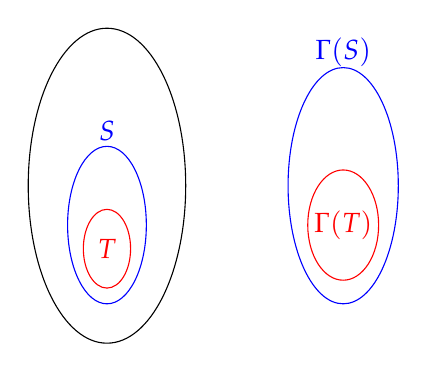
\begin{tikzpicture}
			\draw (0,0) ellipse (1cm and 2cm) ;
			\draw[blue] (0,-0.5) ellipse (0.5cm and 1cm) node[yshift=1.2cm] {$S$};
			\draw[red] (0,-0.8) ellipse (0.3cm and 0.5cm) node {$T$};
			%			\draw[blue] (0,0.5) -- (3,1.5);
			\draw[blue] (3,0) ellipse (0.7cm and 1.5cm) node[yshift=1.7cm] {$\Gm(S)$} ;
			\draw[red] (3,-0.5) ellipse (0.45cm and 0.7cm) node {$\Gm(T)$};
		\end{tikzpicture}
	\end{minipage}
	\vspace{0.5cm}
	
	So $|\Gm^{odd}(S)|>0$. Hence there is a vertex $v\in R$ such that there is odd number of neighbors in $S$. Hence the constraint $v$ is not satisfied. Hence contradiction.\Qed
	
	\parinn
	
	Now let $r$ be the received word and $c\in \mcC(G)$ be the unique codeword such that $\delta(r,c)<\delta(1-2\eps)N$. Denote $$S^{(k)}=\{i\in L\mid x_i^{(k)}\neq c_i\}$$Hence we have $|S^{(0)}|<\delta(1-2\eps)N$. Also we will use the set $\mathsf{UNSAT}^{(k)}$ to denote the set of unsatisfied right constraints at $k$th step. Similarly for $\mathsf{SAT}^{(k)}$. Now we will state the decoding algorithm then we will analyze the algorithm to show the given statement.
		\pagebreak
\section{Decoding Algorithm}
	\begin{algorithm}
		\caption{Linear Time Decoding Algorithm for Expander Code}
		\DontPrintSemicolon
		\KwIn{$r=(r_1,\dots, r_n)$ with promise $\exs!\ c\in \mcC(G)$ such that $\delta(r,c)<\delta(1-2\eps)n$}
		\Begin{
			$k\longleftarrow 0$\;
			$x^{(k)}\longleftarrow r$\;
			\ForEach{$j\in R$}{
				\If{$\sum\limits_{i\in \Gm(j)}x_i=0$}{label $j$ as ``SAT"}
				\Else{label $j$ as ``UNSAT"}
			}
			\ForEach{$i\in L$}{
				$\mathsf{SAT}_i^{(k)}=\{j\in \Gm(i)\mid j\text{ labeled ``SAT"}\}$\;
				$\mathsf{UNSAT}_i^{(k)}=\{j\in \Gm(i)\mid j\text{ labeled ``UNSAT"}\}$\;
			}
			\While{$\exs\ i\in L$  s.t. $|\mathsf{UNSAT}^{(k)}_i|>\frac23|\Gm(i)|$}{
				$x_i^{(k+1)}\longleftarrow 1-x_i^{(k)}$\;
				$x_{i'}^{(k+1)}\longleftarrow x_{i}^{(k)}$ for all $i'\neq i$\;
				Update $\mathsf{SAT}_i^{(k)}$ and $\mathsf{UNSAT}_i^{(k)}$\;
				$k\longleftarrow k+1$\;
			}
			\Return $x^{k}$
		}	
	\end{algorithm}
	
\section{Analysis}
\parinf	
\textbf{\textit{Lemma 2:}} \label{exdecodelem1}
	If $\eps\in\lt( 0,\frac16\rt)$ and $0<|S^{(k)}|\leq \delta N$ then $\exs\ i\in L$ such that $|\mathsf{UNSAT}_i^{(k)}|>\frac23|\Gm(i)|$.


\textbf{\textit{Proof:}} \parinn First notice that all unique neighbors of $S^{(k)}$ are unsatisfied at $k$th iteration. $\eps\in \lt(0,\frac16\rt)$ hence  the graph has $(1-2\eps)D|S|$ unique neighbors for any $S\subseteq L$ with $|S|\leq \delta N$ by \hyperref[p:p2]{Problem \ref{p:p2}} part (1). Hence $$|\mathsf{UNSAT}^{(k)}|\geq |\Gm^+(S^{(k)})|\geq (1-2\eps)D|S^{(k)}|> \frac{2D}{3}|S^{(k)}|$$Hence, $\exs\ i\in S^{(k)}$ such that $|\mathsf{UNSAT}_i^{(k)}|>\frac{2D}3$. Now the degree of $i$ is $D\implies |\Gm(i)|=D$. Hence $|\mathsf{UNSAT}_i^{(k)}|>\frac23|\Gm(i)|$. \Qed

	
\parinf

\textbf{\textit{Observation:}} \begin{itemize}
	\item The number of unsatisfied right constraints is always decreasing.
	\item $|S^{(k)}-S^{(k+1)}|=1$
\end{itemize}

\parinf	

\textbf{\textit{Lemma 3:}}\label{exdecodelem2} $|S^{(0)}|<\delta(1-2\eps)N\implies |S^{(k)}|<\delta N$.


\textbf{\textit{Proof:}} \parinn Initially $\mathsf{UNSAT}^{(0)}\subseteq {\Gm(S^{(0)})}$ since the unsatisfied constraints are the subset of the neighbors of errors. Hence $$|\mathsf{UNSAT}^{(0)}|\leq|{\Gm(S^{(0)})}|\leq D|S^{(0)}|<D|S^{(0)}|<\delta(1-2\eps)DN$$
	
Suppose there exists a $k'$ such that $|S^{(k')}|\geq \delta N$. By the observation there exists $k\leq k'$ such that $|S^{(k)}|=\delta N$. Hence $$|\mathsf{UNSAT}^{(k)}|>|\Gm^+(S^{(k)})|\geq \delta N\cdot (1-2\eps)D$$But the $|\mathsf{UNSAT}^{(k)}|$ keeps decreasing so it can not start with less than $\delta(1-2\eps)DN$ and after that at some point is $\geq \delta N\cdot (1-2\eps)D$. Hence contradiction. \Qed

Since for each iteration the distance between $x^{(k)}$ and $c$ is at most $\delta N$, $c$ is the only codeword which is nearest to $x^{(k)}$. Hence the nearest codeword for each iteration stays the same.

At $k$th iteration  suppose the  number of unsatisfied constraints is nonzero and $|S^{(k)}|<\delta n$. Since number of  unsatisfied constraints is nonzero $|S^{(k)}|> 0$. By \lmref{exdecodelem1}  there exists an $i\in L$ such that $|\mathsf{UNSAT}_i^{(k)}|>\frac23|\Gm(i)|$. Hence the algorithm will find some vertex which has more unsatisfied constraints than satisfied constraints and flip its bit and proceed to the next iteration. With this process the number of unsatisfied constraints reduced by at least 1. Thus the algorithm will keep reducing the number of unsatisfied constraints till it becomes zero because if its not zero at any $j$th iteration and then $|S^{(j)}|>0$ and hence by the above argument it will proceed. Once the  number of unsatisfied constraints becomes zero cause then the final output, suppose $x$ satisfies all the right constraints. Hence it is indeed a codeword and since the nearest codeword at each iteration stays the same $x=c$. 

Therefore the above algorithm can decode with $(1-2\eps)\frac{K}{N}$ fraction errors. Since $(1-3\eps)\frac{K}{N}< (1-2\eps)\frac{K}{N}$ as $\eps\in\lt(0,\frac16\rt)$ as in \lmref{exdecodelem1} we have a $(1-3\eps)\frac{K}{N}$-decoder algorithm. Now in the next section we will prove that it is a polynomial time (in fact linear time) algorithm.

\section{Time Complexity}
\begin{enumerate}
	\item Preprocessing Stage: For each $j\in R$ to check $\sum_{i\in \Gm(j)}x_i=0$ it takes $O(d)$ time. Hence the first for loop takes $O(md)$ time. Now for each vertex in $L$ we keep the number of unsatisfied constraints which are neighbor of that vertex. We also keep a list of vertices in $L$ which have more unsatisfied constraints than satisfied constraints. This can be done in $O(cn)$ time.
	\item In each iteration of the while loop instead of searching for a vertex with more unsatisfied constraints than satisfied constraints we remove an element of $Q$. \parinn
	
	After flipping the vertex we update the list of unsatisfied constraints in $R$ in $O(c)$ time. Then we  will update the number of unsatisfied constraints associated with each element of in $L$ which are neighbors of the neighbors of $i$ i.e. the vertices in  $\Gm(\Gm(i))$ in $O(cd)$ time. Since after the bit flip the previously unsatisfied constraints are satisfied in $\Gm(i)$ and the previously satisfied constraints are now unsatisfied. For each vertex $j\in\Gm(i)$ if $j$ was previously unsatisfied then we will subtract 1 from the number of unsatisfied constrains of the neighbors of $j$ and if $j$ was previously satisfied then we will add 1 for any previously satisfied constraint to the number of unsatisfied constrains of the neighbors of $j$. Now from $Q$ we will remove the elements which have lesser unsatisfied constraints than satisfied constraints and add the.
	
	After updating the number of unsatisfied constraints of each vertex in $\Gm(\Gm(i))$ we will add the vertices which have more unsatisfied constraints than satisfied constraints into $Q$ and remove the vertices which have lesser unsatisfied constrains than satisfied constraints. This all can be done in $O(cd)$ time since $|\Gm(\Gm(i))|\leq cd$. Since $c,d$ are constants every thing inside each iteration can be done in constant time.
	\item In each iteration the number of unsatisfied constraints reduces by at least 1. The original number of unsatisfied constraints is at most $c\delta (1-2\eps)n$. (\lmref{exdecodelem2}). Then the total number of iterations is at most $c\delta(1-2\eps)n=O(n)$.
\end{enumerate}
Hence the algorithm decodes the received word in $O(n)$ time.
\end{enumerate}
}

\pagebreak

%%%%%%%%%%%%%%%%%%%%%%%%%%%%%%%%%%%%%%%%%%%%%%%%%%%%%%%%%%%%%%%%%%%%%%%%%%%%%%%%%%%%%%%%%%%%%%%%%%%%%%%%%%%%%%%%%%%%%%%%%%%%%%%%%%%%%%%%
% Problem 4
%%%%%%%%%%%%%%%%%%%%%%%%%%%%%%%%%%%%%%%%%%%%%%%%%%%%%%%%%%%%%%%%%%%%%%%%%%%%%%%%%%%%%%%%%%%%%%%%%%%%%%%%%%%%%%%%%%%%%%%%%%%%%%%%%%%%%%%%

\begin{problem}{%problem statement
	}{p4% problem reference text
	}
	Write a short analysis of the Zig-Zag product construction the way we used int he algorithm of Reingold
\end{problem}
\solve{
We will show that USTCONN is in log-space. The main observation used here is 

For expander graphs the diameter of the graph is $O(\log N)$ where $N$ is the number of vertices. Then to check $s-t$ connectivity we can start from $s$ and then take all possible $O(\log N)$ length step walks and output `YES' if any of the walks reaches $t$. This uses $O(\log N)$ space as only the index of the vertex for the next step in the current $O(\log N)$ length walk is need to be stored.

For any given graph $G$ we will first convert $F$ to $G'$ which is non-bipartite by just adding self loops for all vertices of $G$. Now if $G'$ is non-regular then we will make the graph 3-regular. For each vertex $v$ in the graph let $d_v$ is the degree of the vertex then we will replace $v$ with a $d_v$ cycle. Now the graph is 3-regular. Let the final graph is $G''$. 

At this point suppose the graph $G''$ is now $D$ regular. Then we take an expander graph $H$ which is $\lt(D^{16},D,\frac12\rt)$. Now we will recursively define a graph family$$G_0=G'',\qquad G_{k}=(G_{k-1}\textcircled{z}H)^8$$Now suppose $\lm_k$ denote the second larges value of $G_k$. And $\lm_H$ denote the second largest eigenvalue of $H$ i.e. $\lm_H=\frac12$. Initially we have by a result of Alon and Sudakov is $\lm_0\leq  1-\frac1{D^{16}N^2}$. Now we have a claim:\parinf

\textbf{\textit{Claim:}} For any $i$, $\lm_i\leq \min\{\lm_{i-1}^2,\frac12\}$.

\textbf{\textit{Proof:}} Using \cite[Theorem 4.3]{reingold2004entropy} we have  $$\lm_{A\textcircled{z}B}\leq \frac12(1-\lm_B^2)\lm_A+\frac12\sqrt{(1-\lm_B^2)^2\lm_A^2+4\lm_2^2}$$In our case $\lm_H\leq \frac12$. So we will have $$\lm_k\leq 1-\frac12(1-\lm_{i-1})(1-\lm_H^2)$$

So we have $$\lm_{G_{i-1}\textcircled{z}H}\leq 1-\frac12(1-\lm_{i-1})(1-\lm_H^2)\leq 1-\frac12\lt(1-\lm_{i-1}\rt)\lt(1-\frac14\rt)\leq 1-\frac12\lm_{i-1}\leq 1-\frac38(1-\lm_{i-1}^2)$$Hence we have $$\lm_i=(\lm_{G_{i-1}\textcircled{z}H})^8\leq \lt(1- \frac38(1-\lm_{i-1}^2)  \rt)$$Now if $\lm_i\leq \frac12$ then $\lm_{i+1}\leq \lt(1-\frac3{16}\rt)^7\leq \frac 12$. And if $\lm_i>\frac12$ then for $x\in\lt[\frac12,1  \rt]$ we have $$\lt(1-\frac38(1-x)\rt)^8\leq \lt( 1-\frac{3}8\times 4(1-x)\rt)^2\leq \lt(1-\frac32(1-x)\rt)^2\leq (1-(1-x))^2= x^2$$Therefore $\lm_i\leq \lm_{i-1}^2$. Hence we always have $\lm_i\leq \min \{\lm_{i-1}^2,\frac12\}$.\Qed

Now $\lm_i\leq \lm_{i-1}^2$. Therefore we have $$\lm_i\leq \lm_0^{2^i}\leq \lt( 1-\frac1{D^{16}N^2}  \rt)^{2^i}\leq \frac 12$$ Hence it is enough to have $i\geq \log (D^{16}N^2\log 2)=O(\log N)$. Therefore if we do this above process $O(\log N)$ many times we will have a good expander then we have the diameter $O(\log N)$.
}
\bibliographystyle{alpha}
\bibliography{refs}
\end{document}
